\documentclass[12pt]{article}
\pdfoutput=1

\usepackage[margin=2.5cm]{geometry}
\usepackage{graphicx}
\usepackage{natbib}
%correct punctuation for MBE
\bibpunct[,]{(}{)}{;}{a}{}{,}

\usepackage{amsmath}

\renewcommand{\bottomfraction}{.9}
\renewcommand{\topfraction}{.9}
\renewcommand{\textfraction}{0.1}
\renewcommand{\floatpagefraction}{.9}

\linespread{1.5}
\begin{document}

\title{\textbf{Predicting virus-receptor mutant binding by molecular dynamics simulation}}
\author{Austin G. Meyer$^{1,2,4*}$, Sara L. Sawyer$^{3}$, Andrew D. Ellington$^{2}$,\\and Claus O. Wilke$^{1}$}
\date{}

\maketitle
\noindent
Address:\\
$^1$Section of Integrative Biology, Institute for Cellular and Molecular
Biology, and Center for Computational Biology and Bioinformatics. The University
of Texas at Austin, Austin, TX 78712, USA.\\
$^2$Department of Chemistry and Biochemistry, Institute for Cellular and Molecular 
Biology, The University of Texas at Austin, Austin, TX 78712, USA.\\
$^3$Section of Molecular Genetics and Microbiology, Institute for Cellular and Molecular 
Biology, The University of Texas at Austin, Austin, TX 78712, USA.\\
$^4$School of Medicine, Texas Tech University Health Sciences Center, 
Lubbock, TX 79430, USA.\\

\bigskip
\noindent
$^*$Corresponding author\\
$\phantom{^*}$Email: austin.meyer@utexas.edu\\
$\phantom{^*}$Phone: +1 512 971 0123\\

\bigskip
\noindent
Manuscript type: research article

\bigskip
\noindent Keywords: protein--protein interaction, molecular dynamics, arenavirus, machupo

\newpage

\begin{abstract}
Existing computational methods to predict protein--protein interaction affinity often perform poorly in important test cases. In particular, the effects of multiple mutations, non-alanine substitutions, and flexible loops are difficult to predict with available tools and protocols. We present here a new method to interrogate affinity differences resulting from mutations in a host-virus protein--protein interface. Our method is based on extensive non-equilibrium all-atom simulations: We computationally pull the machupo virus (MACV) spike glycoprotein (GP1) away from the human transferrin receptor (hTfR1) and estimate affinity using the maximum applied force during a pulling simulation and the area under the force-versus-distance curve. We find that these quantities can provide novel biophysical insight into the GP1/hTfR1 interaction. First, with no prior knowledge of the system we can differentiate among wild-type and mutant complexes. Second, although the static co-crystal structure shows two large hydrogen-bonding networks in the GP1/hTfR1 interface, our simulations indicate that one of them may not be important for tight binding. Third, one viral site known to be critical for infection may mark an important evolutionary suppressor site for infection-resistant hTfR1 mutants. Finally, our method provides an elegant framework to compare the effects of multiple mutations, individually and jointly, on protein--protein interactions.
\end{abstract}

\section*{Introduction}

The computational prediction of mutational effects on protein--protein interactions remains a challenging problem. Several methods are available to perform an energy difference calculation from an experimentally determined co-crystal structure. For example, computational alanine-scanning can be performed rapidly, with relatively low computational cost \citep{Grant2011,Kortemme2004}. However, such methods calculate the relative contribution to overall energy for each amino acid in a protein. They do not probe the interface directly, but rather calculate the total energy with each substitution \citep{Grant2011,Kortemme2004}. Alternative approaches have been developed using machine learning, training coefficients in a weighted equation containing geometric and energetic parameters \citep{Vreven2011,Vreven2012,Bajaj2011,Hwang2010}. Unfortunately, such machine-learning approaches often suffer in novel applications, for which available training sets are small or non-existent. As such, these methods are poorly suited for most host-virus protein--protein systems. By contrast, first principles methods offer the chance to forgo training. However, the currently available methods such as free energy perturbation (FEP) and thermodynamic integration (TI) rely on a two state model (where one state may be wild-type and the other may be a mutant) that transitions directly from one three-dimensional model to another with no intermediate steps \citep{Gilson1997,Lu2004,Chodera2011,Gumbart2013}. As a result, the accuracy of the measurement suffers as the two proteins become increasingly dissimilar; therefore, these techniques are largely limited to point mutant comparisons.

Here we propose a new method to probe mutational effects in protein--protein interactions directly based on first principles simulation, by pulling two proteins apart that are initially bound in a complex. We impart a pulling force within an all-atom molecular dynamics simulation on one member of the complex while the other is held in place. Then, we measure the force required for dissociation \citep{Gumbart2012,Lu1999,Park2004,Is2001A,Is2001B}. As a proxy for relative binding affinity, we use the maximum applied force required for separation and the area under the force-versus-distance curve (AUC). 

We applied our method to interrogate the interaction between machupo virus (MACV) spike glycoprotein (GP1) and the human transferrin receptor (hTfR1) \citep{Abraham2010,Charrel2003}. Machupo is an ambisense RNA virus of the arenavirus family \citep{Charrel2003}. Worldwide, arenaviruses represent a significant source of emerging zoonotic diseases for the human population \citep{Charrel2003}. Members of the arenavirus family include the Lassa fever virus endemic to West Africa, the lymphochoriomeningitis virus (LCMV) endemic to rodents in several areas of the United States, and the Guanarito, Junin, and Machupo viruses endemic to rodents in South America \citep{Charrel2003}. The South American arenaviruses typically infect humans after rodent contamination and can cause a devastating hemorrhagic fever with high mortality \citep{Charrel2003}.

The hTfR1 is the primary receptor used by MACV for binding its host cell prior to infection. The primary role of hTfR1 $in~vivo$ is to bind transferrin for cellular iron uptake. The hTfR1 protein contains three extracellular domains: two basilar domains and an apical domain. The two basilar domains serve most of the transferrin-binding function \citep{Abraham2010,Rad20112}. Viral entry is initiated by GP1 binding to the apical domain of hTfR1. Previous work has indicated that the GP1/hTfR1 binding interaction is the primary determinant of MACV host range variation \citep{Rad20111,Rad20112}. The co-crystal structure shows the high affinity interaction between GP1 and hTfR1 forces the normally flexible loop in the apical domain of hTfR1 into a rigid beta-pleated sheet domain. For GP1, several extended loops in mediate binding to hTfR1 \citep{Abraham2010,Rad20112}, and many of the interface interactions are mediated by extensive hydrogen-bonding networks \citep{Abraham2010}. Experimental alanine-scanning and whole cell infectivity assays have identified several sites in both GP1 and hTfR1 that are probably critical for establishing infection \citep{Rad20111,Rad20112}.

We applied our computational method to wild type (WT) and mutant complexes, and found that we could resolve relative differences in unbinding and predict significant affinity changes. At sites known to be important for successful viral entry, we found that the biochemical cause of reduced infectivity may not be as simple as the static structure suggests. For example, the static structure shows a hydrogen-bonding network connected to site Asn348 in hTfR1. According to our simulations, this network may not affect binding affinity directly. In addition, our study offers an all-atom steered molecular dynamic approach to avoid the pitfalls of several existing methods used to evaluate mutations in protein--protein interfaces.

\section*{Materials and Methods}

\subsection*{System Modeling}

We used the protein visualization software PyMOL \citep{PyMOL} to remove residues 121-190, 301-329, and 383-756 in the hTfR1. No residues were removed from the viral protein. We also removed 10 sugar residues from the native structure.

After system reduction, the Visual Molecular Dynamics (VMD) \citep{Humphrey1996} package along with its system of back-ends was used for all subsequent modeling. The Orient add-on package allowed us to rotate the system axis such that the direction of steering was oriented directly down the z-axis. De-glycosylation simplified the system such that Autopsf could easily find the chain terminations and patch them appropriately. The Solvate package was used to generate a TIP3P water model with a 5 \AA ngstrom buffer (relative to the maximum dimensions of the proteins) on all sides except down the positive z-axis where a 20 \AA ngstrom buffer was created. Finally, we used the Autoionize package to place 150 millimolar NaCl and neutralize the total system charge. In the end, each modeled system had approximately 28,000 atoms.

\subsection*{Equilibration}

NAMD was used for all simulations in this study \citep{Phillips2005}. In addition to the modeled system, for equilibration we generated a configuration file that fixed the $\alpha$-carbon backbone. This was accomplished by setting $\beta = 1$. Further, we generated a configuration file with fixed $\alpha$-carbon atoms at residues 41-92 (numbered linearly, in this case, starting at 1 for the first amino acid as was required for VMD) in the hTfR1. The second file was used to affix a harmonic restraint, thus preventing any unfolding due to system reduction. More importantly, the harmonic restraint allowed the protein complex to equilibrate while preventing any drift from its predefined orientation. Finally, we calculated the system center and dimensions for use in molecular dynamics settings.

We used the Charmm27 \citep{Brooks1983} all-atom force field. The initial system temperature was set to 310K. Several typical MD settings were used including switching and cutoff. In addition, we used a 2 femtosecond time step with rigid bonds (the exact configuration is provided in the supplement). We used periodic boundary conditions with the particle mesh ewald (PME) method of computing full system electrostatics outside of the explicit box. Furthermore, we used a group pressure cell, flexible box, and langevin piston during equilibration. Finally, a harmonic restraint (called harmonic constraint in VMD) was set as stated previously.

To start the simulation, the langevin piston was switched off and the system was minimized for 1000 steps. Next, the fixed backbone was released, and the system was minimized for an additional 1000 time steps. Subsequently, the system was released into all-atom molecular dynamics for 3000 steps. Finally, the langevin piston was turned on and the system was simulated for 2 ns (1,000,000 steps) of chemical time. For each mutant, twenty independent replicates were run with an identical protocol.

\subsection*{Steered Molecular Dynamics}

Following equilibration, the final state of each simulation was used to generate a configuration file fixing the $\alpha$-carbon on residues 1, 58, 73-83, 96, 136, 137, 138, and 161 (again with linear numbering) in the hTfR1. Also, the $\alpha$-carbon of all residues (163-318 in linear numbering) in the GP1 were given an occupancy of 1, indicating they had an applied force during the simulation. 

In every way possible the subsequent steering simulation had the same parameters as the equilibration simulation. Thus, the steered molecular dynamics (SMD) \citep{Is2001A,Is2001B} simulation was a typical restart with slightly different settings. Periodic boundary conditions were incorporated as part of the system and PME was again used to approximate full system electrostatics. In addition, we first tuned the pulling velocity for practical time considerations. Subsequently, the spring constant was adjusted to ensure a sufficient signal-to-noise ratio with the given velocity. As a result, the spring constant was set to 5~kcal/mol/\AA$^2$, velocity set to 1~\AA/ns, and direction down the positive $z$-axis.

Finally, SMD was run for 15 ns (7,500,000 time steps) of chemical time. For each simulation, we randomly selected one of the equilibration runs for restart. We ran 50 replicate simulations per mutant for a total of 550 SMD simulations. All GP1/hTfR1 complexes separated by greater than 4 \AA\ and many separated to 10 or more.

To leave the final trajectory of a tractable size, only 1000 evenly spaced frames were retained from each simulation, leaving a final trajectory size of 323 MB. See the supplemental movie for a representative unbinding trajectory. Initial development of the SMD protocol was carried out on the Lonestar cluster at the Texas Advanced Computing Center (TACC). All production SMD simulations were performed on the Hrothgar cluster at Texas Tech University, using NAMD 2.9. Each simulation was parallelized over 60 computational cores and utilized approximately 20 hours of computing time. The total chemical time simulated for this project was nearly 10 $\mu$s, requiring slightly over 1 million cpu-hours.

\subsection*{Post-processing}

The python packages MDAnalysis \citep{Agrawal2011} and ProDy \citep{Bakan2011} were both used at various points in post-processing. The molecular trajectory (comprising the atomic coordinates per time) was parsed to compute the center-of-mass for each of the two complexes. The starting center-of-mass distance was set to zero and the distance was re-computed at each time step relative to the starting distance. The force is output directly to the standard log file.

The statistical package R was used for all further analysis and visualization. Each of the 50 independent trajectories per mutant produced a fairly noisy force curve. To reduce the noise, we averaged each point with a 50 point interpolation window. The window ensured that the averaged maximum applied force was never cut off near the beginning of the simulation due to lost time steps (caused by averaging). The two primary descriptive statistics we used were maximum interpolated applied force and total area under the interpolated curve (AUC). We used the pairwise.t.test function with the FDR p-value correction to test for significance. The ggplot \citep{ggplot} package was used to generate most of the figures. 

\section*{Results}

\subsection*{The GP1/hTfR1 system}
The GP1/hTfR1 interface marks a particularly important and useful test system. There are several sites on both the human and viral protein known to affect the infectivity phenotype of MACV. Virtually all of the important sites have been mapped by \textit{in vitro} flow-cytometry based entry assays. The GP1/hTfR1 interface appears not to be dominated by one particular type of interaction (electrostatics, hydrogen-bonding, or van der Waals). In addition, much of the binding domain on hTfR1 is on a flexible loop and undergoes a large structural rearrangement upon binding, making many other computational techniques \citep{Grant2011,Kortemme2004} only marginally useful. The complex nature of this interface represents a particularly difficult challenge for traditional computational analysis. 

For our experiments, we used the experimentally determined GP1/hTfR1 structure (PDBID: 3KAS) \citep{Abraham2010}. The apical domain of hTfR1 interacts directly with GP1 while the other two domains are closer to the cell membrane and have essentially no interaction with GP1. The biophysical independence of the apical domain allowed us to isolate it without significantly affecting the GP1/hTfR1 interaction. Figure~\ref{fig:protein_comparison} shows a model of the initial structure and that of the pared structure. Although GP1 has several glycosylatable residues, we opted to use the de-glycosylated protein for this study. The complexity of correctly parameterizing diverse sugar moieties is outside of the scope of this paper. Furthermore, although it is known that GP1 is glycosylated, and some of those sugars contact hTfR1, the effect of those contacts \textit{in vivo} is still unresolved \citep{Abraham2010}.

In total, we tested 7 point mutants and 3 double mutants in addition to the WT complex (Table~\ref{tab:summary_mutants} and Figure~\ref{fig:mutant_comparison}). Mutations at site hTfR1 site 211 have proven capable of causing loss-of-entry according to \textit{in vitro} flow-cytometry infection assays or known host-range limitations \citep{Rad2008,Rad20111,Rad20112}. Most likely, this effect is caused by the destruction of a critical hydrogen bond to Ser113 or Ser111 in GP1. The lost hydrogen bond would lead to the subsequent loss of a large hydrogen-bonding network seen in the crystal structure (Table~\ref{tab:summary_mutants}) \citep{Abraham2010}. In a manner similar to site 211, Asn348 appears to be important for binding by participating in a critical hydrogen bonding network \citep{Rad2008,Abraham2010} to GP1. In particular, Asn348Lys is reported in the literature to cause significantly reduced viral entry \textit{in vivo} (Table~\ref{tab:summary_mutants}) \citep{Rad2008,Abraham2010}. Finally, an alanine mutation at site 111 in GP1 has also been shown to cause decreased entry (Table~\ref{tab:summary_mutants}) \citep{Rad20112}. For notation purposes, the viral site is always referred to with a preceding `v'.  

\subsection*{Steered molecular dynamics simulations}
To ensure a natural solution structure, we performed an initial equilibration phase to reduce the intrinsic crystallization distortions. First, we generated a physically realistic simulation world around the protein complex. The environment included an explicitly modeled bath of water, and a physiologically relevant concentration of ions. Next, we carried out successive rounds of energy minimization with a fixed $\alpha$-carbon backbone, followed by heating, and backbone release. Last, we performed a short round of all-atom molecular dynamics with minimal restraints \citep{Cuendet2008}. We used the final state from each equilibrated system to restart another MD simulation. For SMD, at the centroid of several atoms a force was applied to a single point in GP1. By using a known spring constant, and pulling with a constant velocity, we could calculate the applied force during protein--protein dissociation \citep{Cuendet2008,Cuendet2011}. A typical averaged force curve comparison can be seen in Figure~\ref{fig:force_curve}. The force curves for each mutant were smoothed either by averaging over many replicates as in Figure~\ref{fig:force_curve} or by selecting an interpolation window for averaging. The latter approach was used for statistical analysis. In addition, to minimize the computational time in unproductive molecular dynamics, we shortened the simulation time such that the interaction just barely dropped to zero near the end of each run. As seen in Figure~\ref{fig:force_curve}, this distance was relatively consistent among mutants. The supplementary movie visually illustrates the separation distance between peptide domains. The quantities maximum applied force and AUC were derived from the force versus distances curves. Their summary statistics are reported in Table~\ref{tab:summary_statistics}. As we are more interested in the phenotypic impact of interface mutations we avoided many of the more physically rigorous, but technically complicated calculations that are possible with SMD \citep{Is2001A,Is2001B}.

Before systematically applying SMD to the GP1/hTfR1 interaction, we needed to ensure the method was sufficiently sensitive to distinguish between relatively minor point mutations. While SMD has been applied previously to measure the binding energy of high-affinity T-cell receptor interactions \citep{Cuendet2008,Cuendet2011}, to our knowledge the method has never been used previously to parse small differences in a complex energy landscape. For this initial sensitivity analysis, we tested alanine substitutions congruent with the traditional experimental and computational approach. 

We found that relative to WT, one alanine mutation (Tyr211Ala) produced a very large and statistically significant difference in the maximum applied force and AUC (Figure~\ref{fig:force_curve}, Table~\ref{tab:MAF_pairwise}), while the other two did not (Table~\ref{tab:MAF_pairwise}). When considering additional mutants (also discussed below), we found that maximum applied force was generally sufficient to distinguish mutants (Tables~\ref{tab:MAF_pairwise} and ~\ref{tab:MAF_p}), and AUC was able to add a few more statistically significant differences (Table~\ref{tab:AUC_p}). In general, however, maximum applied force seemed to be the more sensitive statistic than AUC.

\subsection*{Comparative analysis of the GP1/hTfR1 interface}
Considering the involvement of extended hydrogen-bonding networks in the GP1/hTfR1 interface, it was not clear that individual alanine mutations, even those that should destroy such networks, would significantly change the strength of interaction. One major advantage of first principles simulations is the ability to test mutations other than alanine without additional underlying assumptions in the energy function. Seen in Table~\ref{tab:summary_mutants}, we made additional mutations based on biochemical intuition or available experimental data to chemically diverse amino acids including tryptophan, lysine, aspartate, and threonine. Several mutations caused significant relative affinity changes. In addition, to detect synergistic effects, we tested several double mutants where both mutations appeared to cause similar changes in binding. Then, we compared the size of those differences to single mutants (Figure~\ref{fig:sensitivity} and ~\ref{fig:mutant_comparison}).

Although Tyr211Ala appears to have a large impact on binding affinity, no single mutant can provide enough evidence to understand the biochemical difference in binding mechanism. Since alanine is both smaller than tyrosine and also incapable of participating in hydrogen-bond interactions, we tested further mutations to identify the critical biochemical difference responsible for change in binding affinity. In particular, we substituted smaller side chains that, like tyrosine, were capable of hydrogen bonding. We chose Tyr211Asp and Tyr211Thr, two mutations that have been discussed in the context of selection pressure on hosts in rodent populations \citep{Rad2008,Rad20111,Rad20112}. Both mutations proved capable of causing a significant change in binding affinity in our simulations, but the change appeared to be increased affinity (Figure~\ref{fig:sensitivity} and ~\ref{fig:mutant_comparison}, and Table~\ref{tab:MAF_p}).

We also simulated several point mutations at Asn348 in the hTfR1. As discussed above, the alanine mutation at this site showed no significant difference in maximum applied force or AUC from WT (Tables~\ref{tab:MAF_p} and ~\ref{tab:AUC_p}). In addition, neither the Asn348Lys nor the Asn348Trp mutation showed a significant difference from WT. For both of these mutations, however, mean maximum applied force and mean AUC was lower than for WT (See Table~\ref{tab:summary_statistics}).  On the other hand, there was a detectable difference between Asn348Ala and Asn348Lys (Tables~\ref{tab:MAF_p} and~\ref{tab:AUC_p}), with Asn348Lys being a weaker binder. Moreover, Asn348Trp showed nearly identical results to Asn348Lys. The mutations to large amino acids (Asn348Trp and Asn348Lys) produced nearly identical affinity changes, whereas the mutations to amino acids not capable of hydrogen bonding (Asn348Ala and Asn348Trp) produced significantly different affinity changes (Table~\ref{tab:MAF_pairwise}). To check the consistency of our results, we hypothesized that the combination of Tyr211Ala and Asn348Trp, being chemically disconnected in two different hydrogen-bonding networks, would lead to a synergistic loss-of-binding. As expected, the double mutant was the weakest binding mutant tested ($ p < 10^{-6} $) (Tables~\ref{tab:MAF_p} and~\ref{tab:AUC_p}) in this study. Further, according to maximum applied force (but not AUC), the combination of Tyr211Ala and Asn348Trp also showed significantly weaker binding than Tyr211Ala by itself (Tables~\ref{tab:MAF_p} and~\ref{tab:AUC_p}). We suspect that the effect of Asn348Trp alone is near the limit of detection using our method. A larger number of replicates would possibly have resolved affinity differences between Asn348Trp and WT or other mutants more consistently.

Last, we further analyzed a single mutation in GP1, vArg111Ala. As mentioned in the previous subsection, in our simulations this mutant showed no significant change in either maximum applied force or AUC (Tables~\ref{tab:MAF_p} and~\ref{tab:AUC_p}), even though both quantities were, on average, lower than in WT (Table~\ref{tab:summary_statistics}). This result was somewhat surprising, since Tyr211Ala, presumably disrupting the same hydrogen-bonding network as vArg111Ala, displayed a significant reduction in affinity. To probe the interaction between position 111 in the GP1 and position 211 in the hTfR1 further, we also tested the double mutant vArg111Ala/Tyr211Ala. This double mutant showed affinity indistinguishable from WT and significantly higher than Tyr211Ala alone  (Table~\ref{tab:MAF_pairwise}). This result shows that the two sites do indeed interact, and that replacing the hydrogen-bonding network at these sites with a hydrophobic interaction could lead to comparable binding affinity.

\section*{Discussion}

We have applied a method utilizing steering forces in all-atom molecular dynamics simulations to evaluate the effects of mutations at the GP1/hTfR1 interface. We modeled mutations at several sites in the GP1/hTfR1 interface, and verified that our computational protocol was sensitive enough to distinguish point mutants in hTfR1. Further, we identified two test statistics, maximum applied force and AUC, that can be used as proxies for binding affinity. We systematically tested several point mutations to understand their contribution to the binding interaction. In the case of Asn348Lys, we have shown that the static structure provides little insight into why this mutation causes loss-of-infectivity \textit{in vivo}. While Asn348 appears to be involved in a hydrogen-bonding network in the static structure, change in binding at that site may actually be caused by size and charge restriction. We also found that a negatively polar residue at site 211 in hTfR1 is absolutely critical for a tight binding interaction. Any non-polar mutation at Tyr211 in hTfR1 is likely to completely halt viral entry and dramatically decrease the chances of MACV infection.

By extending the SMD technique to investigate a protein--protein interaction we have, in many ways, changed the scope of its application. Traditionally this technique has been either applied to compute equilibrium quantities via a non-equilibrium approximation \citep{Park2003,Park2004,Giorgino2011}, used to estimate protein stability through unfolding \citep{Lu1999}, or used to calculate the absolute free energy of small molecule ligand binding \citep{Dixit2001}. Likewise, others have used SMD to understand the process of binding and unbinding at a resolution unmatched by experiment \citep{Cuendet2011,Giorgino2011}. And still others aimed at more esoteric problems, such as applying driving forces to untie polypeptide knots in toy systems \citep{Sulkowska2010}. Here, we have shown that SMD can provide insight into the \textit{relative} strength of protein--protein interactions. In contrast to more traditional absolute affinity calculations, relative binding is much more useful for experimental application. Further, our method complements whole cell infectivity assays, which demonstrate phenotypic effects but do not provide biochemical mechanisms. Via SMD, one can separate mutations whose likely effect is altered binding affinity from mutations that may affect other factors such as protein expression, protein folding, or interactions with other proteins not considered in the simulation. Thus, SMD may open avenues for subsequent experimental work.

Our findings may rationalize several effects observed in both infectivity data and rodent populations \citep{Rad2008,Rad20111}. First, we found that some substitutions at positions 211 and 348 did affect the strength of receptor binding. However, the computational data suggest that the reason and nature of the effects at these two sites are very different. At position 211, mutations to non-polar residues causes a large change in binding. This is congruent with what is known from viral entry data \citep{Rad2008,Rad20111}. By contrast, mutations at position 348 need only be small to maintain WT binding. The ability to hydrogen bond appears to be insignificant. This can be inferred from the fact that Tyr211Ala paired with large (Trp) and positively charged (Lys) substitutions at position 348 results in a larger than expected synergistic difference. That is, the double mutant Tyr211Ala/Asn348Trp caused a much larger decrease in binding than we expected from either mutation individually. Third, the GP1 mutation vArg111Ala causes a loss-of-infection during \textit{in vitro} infectivity assays \citep{Rad20112}, yet it was indistinguishable from the WT complex in our simulations. Although Tyr211Ala was the most disruptive single mutant we tested, vArg111Ala in the GP1 was able to restore mean maximum applied force to WT levels (Table~\ref{tab:summary_statistics}), and to levels significantly higher than observed for Tyr211Ala alone.

We would like to emphasize here that we cannot expect perfect agreement. While we have shown that our method can distinguish individual point mutations, we do not know the limit of detection with our method. First, it is possible that some mutants display measurable phenotypic effects in experiments yet appear identical under our method. More extensive sampling or refinement of the simulation protocol could help to differentiate such mutants (see also next paragraph). Second, our SMD method is fundamentally a measurement tool, and as a result we are dramatically limited by the accuracy of our starting structure. Third, the available experimental data for the GP1/hTfR1 system were generally obtained from entry assays or whole-cell binding assays rather than molecular binding assays. A mutant may cause a phenotypic difference in infectivity without generating a signal by our method. For example, entry could be lost in the experimental system because the protein is grossly or partially misfolded. An additional analytical step with circular dichroism or an analogous technique could clarify such large-scale folding differences. Further, since our simulations start with a bound structure, any changes that may dramatically affect the rate of association (different folds, trafficking issues, etc.) or relative orientation of the two proteins would be underestimated by our method. Finally, it is tempting to think only decreased binding affinity should correlate strongly with diminished infectivity. However, dramatically increased binding affinity could also disrupt infectivity by prohibiting cellular membrane detachment after viral invasion. The virus would be prevented from reaching its replication compartment (which is the cytosol in the case of Machupo) and could not reproduce.

There are a few additional challenges for investigating host-virus interaction via molecular dynamics simulation. As with any atomistic simulation, there is going to be a fairly large noise to signal ratio. To reduce noise, one could further customize each simulation, e.g. by determining the optimal pulling speed. Furthermore, larger amounts of computational resources will have a direct and powerful impact on the strength of any atomistic study \citep{Shaw2012}. Such resources could come in the form of increased compute time, improved code, or customized hardware for floating point operations \citep{Shaw2011}. With improved resources, we could investigate thousands of individual permutations in the GP1/hTfR1 binding interface. In addition, with additional compute time it would be possible to incorporate equilibrium sampling approaches \citep{Buch2011} or use brute force equilibrium approaches \citep{Giorgino2012} to improve resolution. Going forward, we believe that all-atom molecular dynamics simulations can become an increasingly viable approach for protein interaction studies. 

\section*{Acknowledgments}
This work was carried out using high-performance computing resources provided by the High Performance Computing Center (HPCC) at Texas Tech University at Lubbock (http://www.hpcc.ttu.edu) and the Texas Advanced Computing Center (TACC) at The University of Texas at Austin (http://www.tacc.utexas.edu). The authors acknowledge Bryan Sutton for opening access to the Hrothgar cluster.

This work was supported by the Defense Threat Reduction Agency (HDTRA1-12-C-0007) to A.D.E., S.L.S., and C.O.W., the National Science Foundation (MCB-0943383) and the Welch Foundation (F-1654) to A.D.E., the National Institutes of Health (R01-GM088344) to C.O.W., and the National Institutes of Health (R01-GM093086) to S.L.S.

\bibliographystyle{MBE}
\bibliography{paper}

\clearpage
\begin{figure}[p]
\centerline{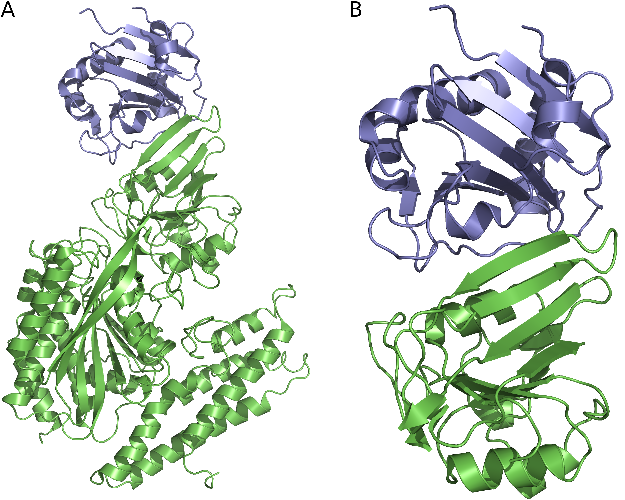
\includegraphics[width=6in]{figures/protein_comparison.pdf}}
\caption{\label{fig:protein_comparison}\title{The GP1/hTfR1 complex.} GP1 is shown in blue and hTfR1 is shown in green. (A) The full, de-glycosylated GP1/hTfR1 co-crystal structure. (B) The reduced structure used in SMD simulations.}
\end{figure}

\clearpage
\begin{figure}[p]
\centerline{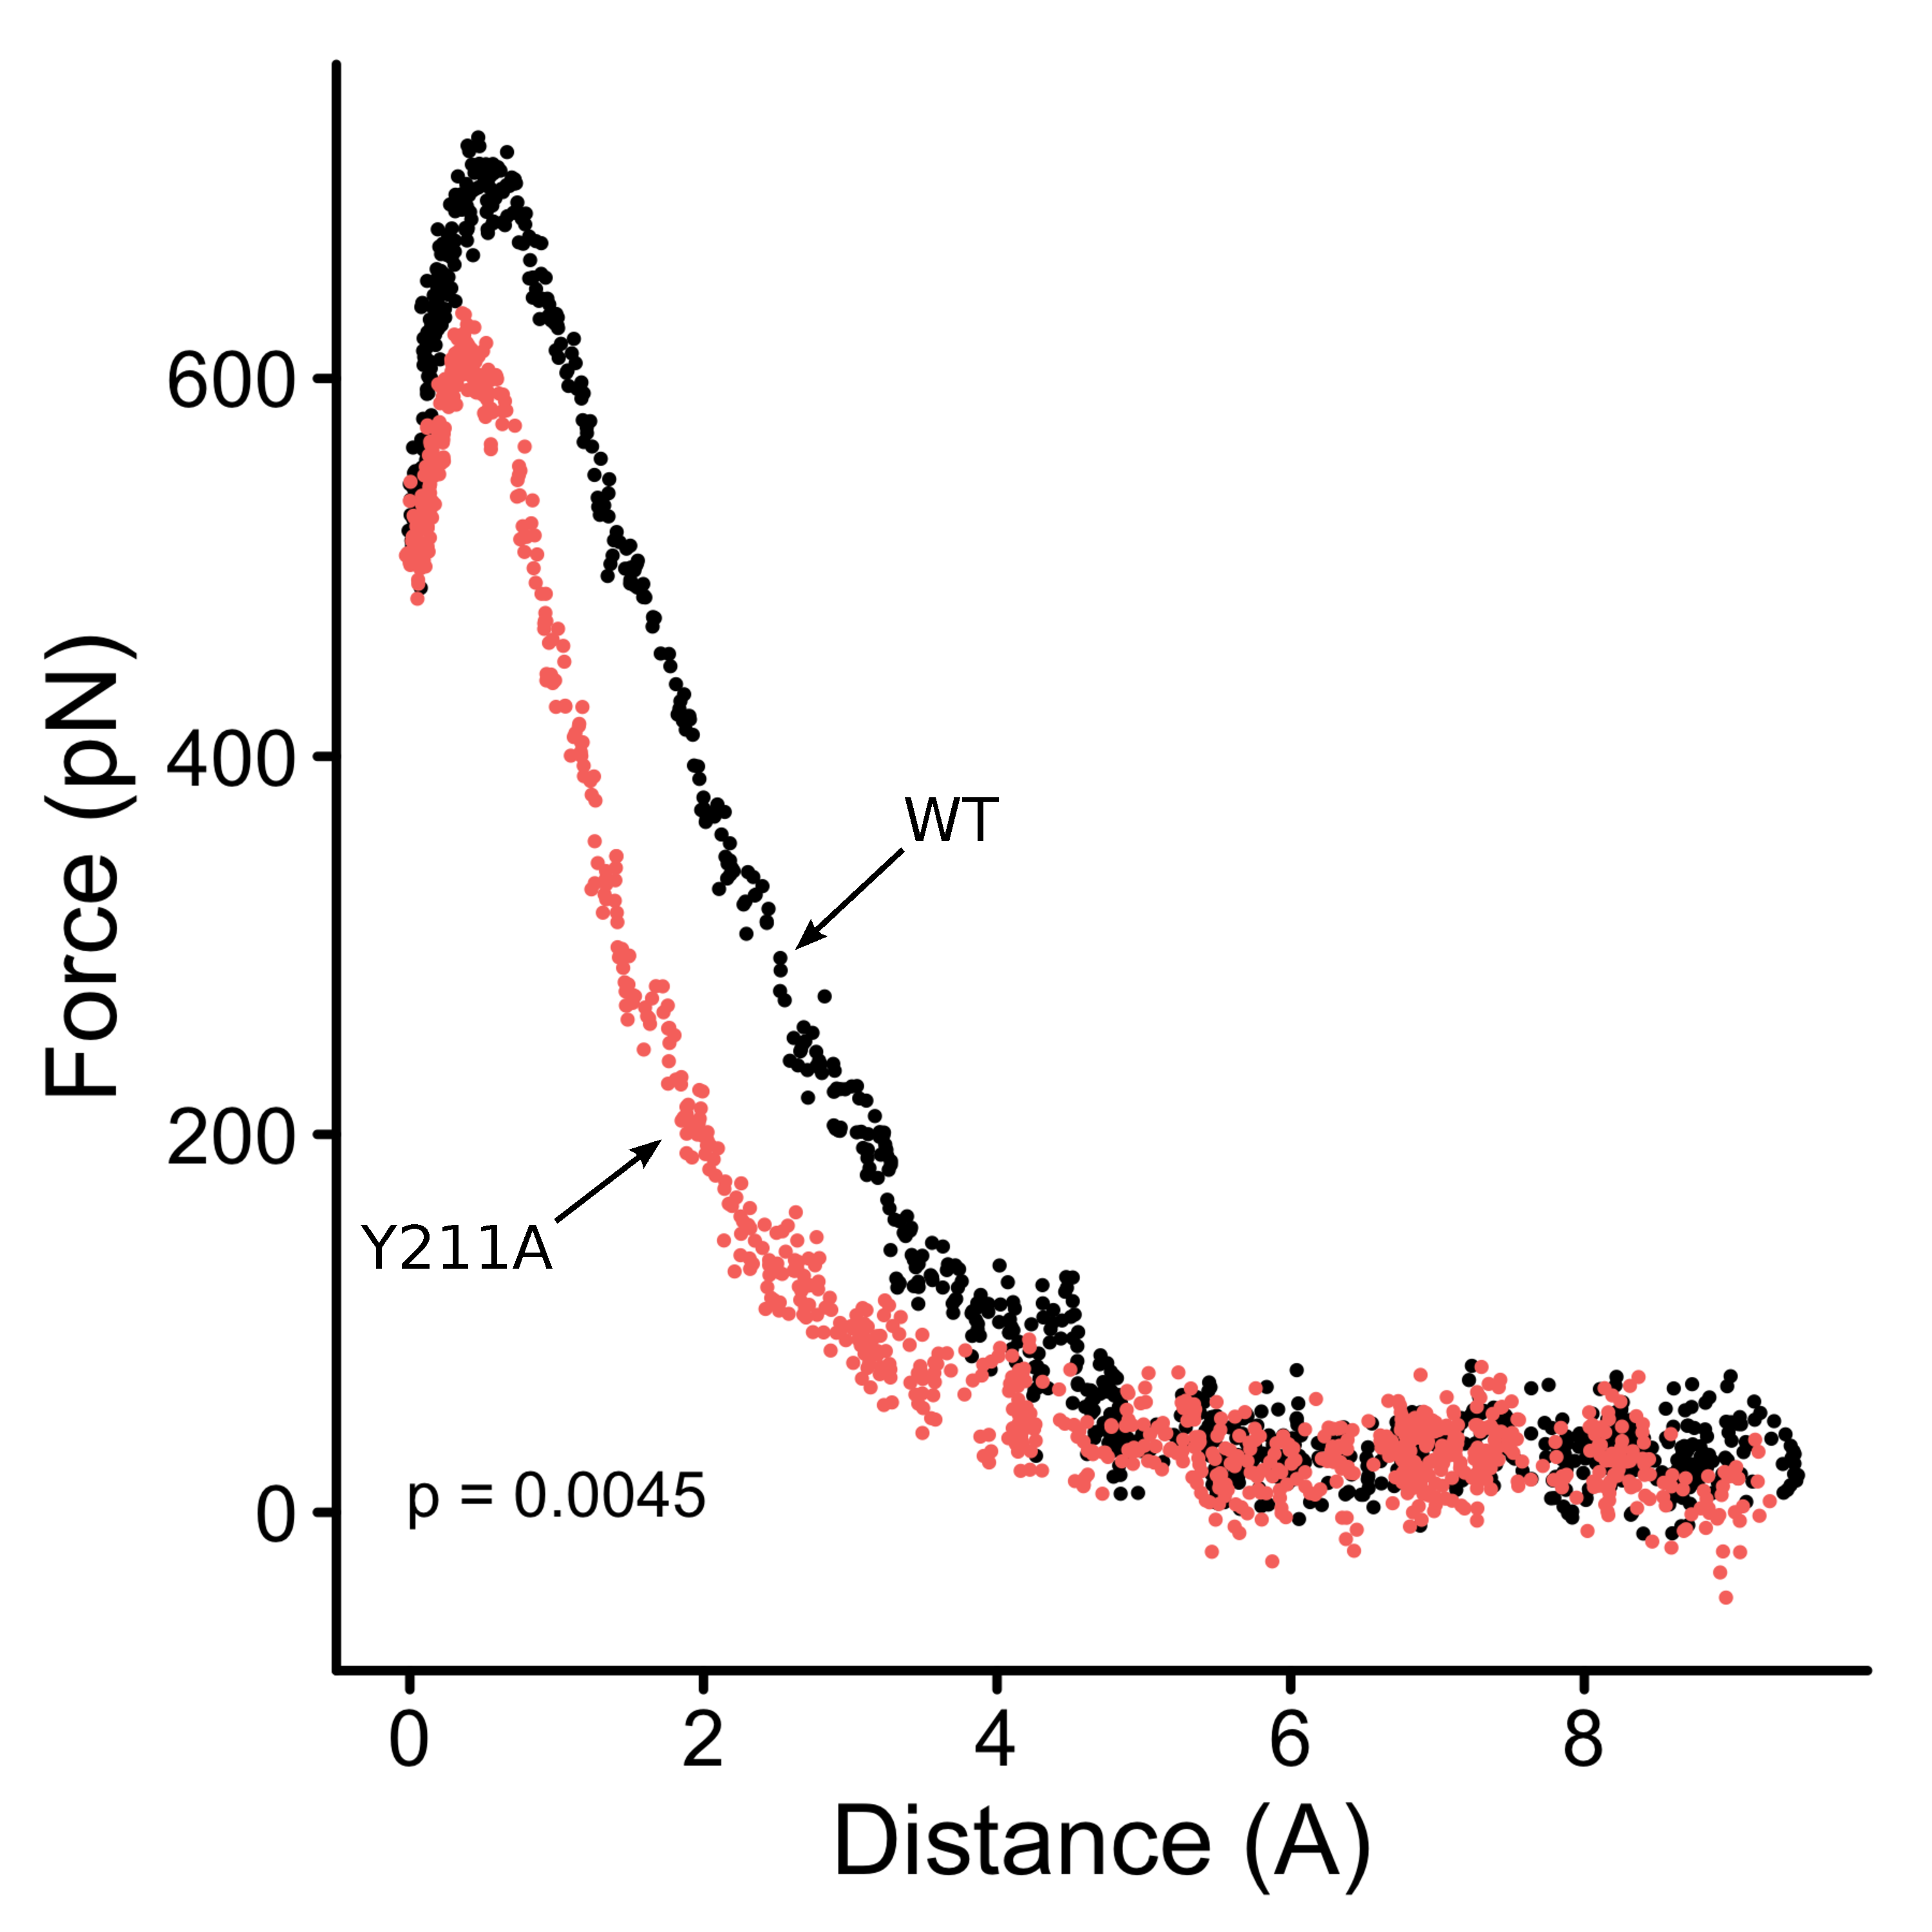
\includegraphics[width=6in]{figures/force_curve.pdf}}
\caption{\label{fig:force_curve}\title{Force versus distance curve of WT and the Y211A mutant.} The average force curve for 50 replicates of the WT complex is shown in black, and the average of 50 replicates of the Y211A mutant is shown in red. There is a large difference in both maximum applied force and AUC between the two complexes.}
\end{figure}

\clearpage
\begin{figure}[p]
\centerline{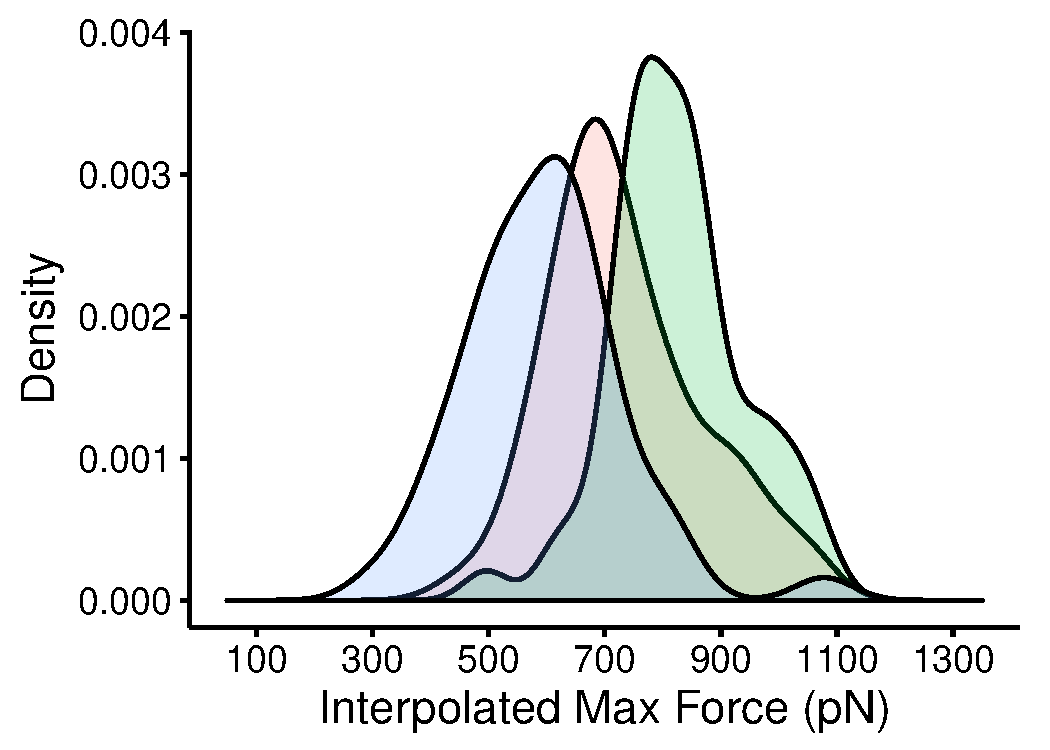
\includegraphics[width=6in]{figures/sensitivity_histogram.pdf}}
\caption{\label{fig:sensitivity}\title{Distribution of interpolated maximum force for three different GP1/hTfR1 complexes.} The WT GP1-hTfR1 complex in the middle is flanked by the tighter binding mutant Y211D on the right and the weaker binding double mutant N348W/Y211A on the left. The large non-overlapping areas indicate a large and statistically significant difference in these three complexes.}
\end{figure}

\clearpage
\begin{figure}[p]
\centerline{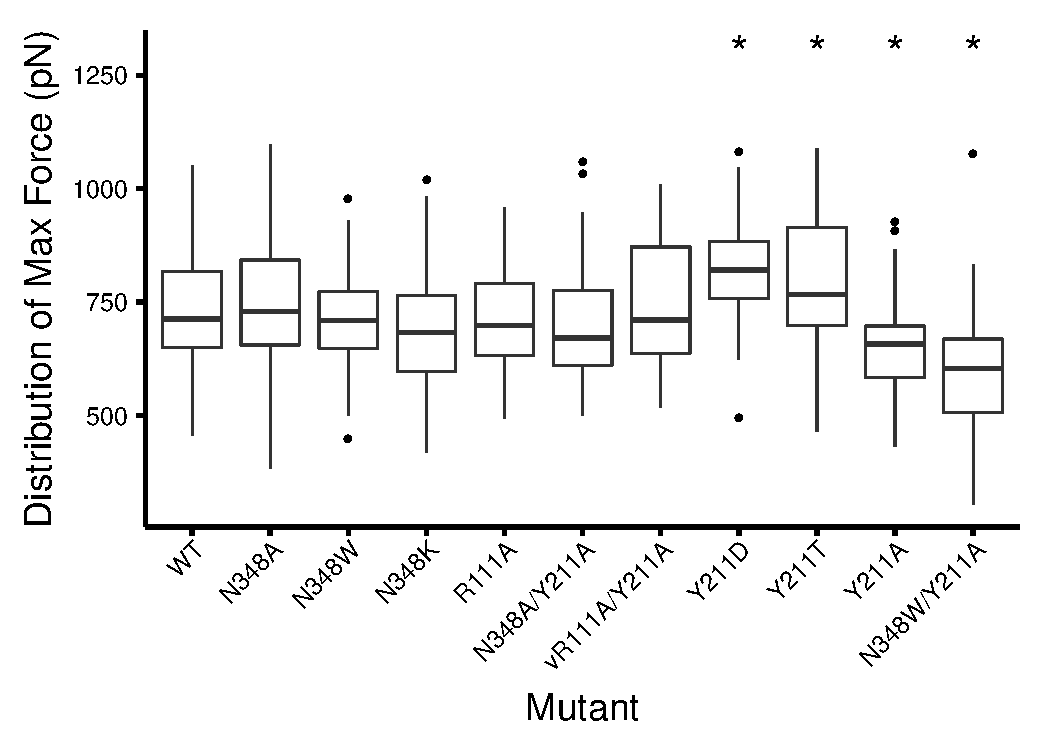
\includegraphics[width=6in]{figures/mutant_comparison_boxplot.pdf}}
\caption{\label{fig:mutant_comparison}\title{Distribution of interpolated maximum force for all complexes tested.} The statistically significant difference relative to the WT complex are indicated by a star above the distribution.}
\end{figure}

\clearpage
\begin {table}[H]
\caption{\label{tab:summary_mutants}Summary of information for each mutation tested. Observed $in~vivo$ refers to mutations that have been observed in rodent populations. Phenotype $in~vitro$ refers to the observed phenotype in $in~vitro$ viral entry assays.} 
\begin{center}
  \resizebox{11cm}{!} {
    \begin{tabular}{l c r r}
    \hline
      Mutation & Observed $in~vivo$ & Phenotype $in~vitro$ \\
            WT &                Yes &         Normal Entry \\
         N348A &                 No &                    - \\
         N348K &                Yes &     Diminished Entry \\
         N348W &                 No &                    - \\
         Y211A &                 No &        No Expression \\
         Y211D &                Yes &        No Expression \\
         Y211T &                 No &     Diminished Entry \\
        vR111A &                 No &     Diminished Entry \\
   N348A/Y211A &                 No &                    - \\
   N348W/Y211A &                 No &                    - \\
  vR111A/Y211A &                 No &                    - \\
    \hline
    \end{tabular}
  }
\end{center}
\end{table}

\clearpage
\begin {table}[H]
\caption{\label{tab:summary_statistics}Summary statistics for each mutation tested. $\mu_\text{MAF}$ is the mean and $\sigma_\text{MAF}$ is the standard deviation of maximum applied force over all simulations. $\mu_\text{AUC}$ is the mean and $\sigma_\text{AUC}$ is the standard deviation of AUC over all simulations.}
\begin{center}
  \resizebox{11cm}{!} {
    \begin{tabular}{l r r r r}
    \hline
      Mutation &      $\mu_\text{MAF}$ & $\sigma_\text{MAF}$ & $\mu_\text{AUC}$ & $\sigma_\text{AUC}$ \\ \hline
            WT &                772.00 &              154.13 &         198794.7 &            66765.64 \\
         N348A &                799.33 &              154.36 &         202247.3 &            65175.78 \\
         N348K &                731.36 &              151.01 &         179087.5 &            55799.49 \\
         N348W &                732.13 &              131.21 &         192043.2 &            66916.36 \\
         Y211A &                684.03 &              126.69 &         153517.7 &            40889.12 \\ 
         Y211D &                875.44 &              116.46 &         234909.3 &            50494.11 \\ 
         Y211T &                861.17 &              158.48 &         231078.7 &            97569.29 \\
        vR111A &                754.39 &              103.25 &         185896.8 &            46408.74 \\
   N348A/Y211A &                762.96 &              144.81 &         173059.2 &            59898.10 \\
   N348W/Y211A &                617.21 &              163.33 &         147705.6 &            48548.61 \\
  vR111A/Y211A &                780.71 &              135.65 &         189919.1 &            48868.16 \\
    \hline
    \end{tabular}
  }
\end{center}
\end{table}

\clearpage
\begin {table}[H]
\caption{\label{tab:MAF_pairwise}Pairwise differences (row variable minus column variable) in mean maximum applied force. Bolded values are statistically significant at $p<0.05$. Values marked with * and ** are significant at $p<0.01$ and $p<0.001$, respectively.}
\begin{center}
  \resizebox{16cm}{!} {
    \begin{tabular}{l l l l l l l l l l l}
    \hline
                & WT                  & N348A              & N348W              & N348K              & Y211A             & Y211D              & Y211T              & vR111A             & N348A/Y211A        & N348W/Y211A        \\ \hline
    N348A       &  27.33              &                    &                    &                    &                   &                    &                    &                    &                    &                    \\
    N348W       & -39.87              & \textbf{-67.20}    &                    &                    &                   &                    &                    &                    &                    &                    \\
    N348K       & -40.64              & \textbf{-67.97}    & -0.77              &                    &                   &                    &                    &                    &                    &                    \\
    Y211A       & \textbf{-87.97*}    & \textbf{-115.30**} & -48.10             & -47.33             &                   &                    &                    &                    &                    &                    \\
    Y211D       & \textbf{103.44**}   & \textbf{76.12*}    & \textbf{143.31**}  & \textbf{144.08**}  & \textbf{191.42**} &                    &                    &                    &                    &                    \\
    Y211T       & \textbf{89.17*}     & \textbf{61.85}     & \textbf{129.04**}  & \textbf{129.81**}  & \textbf{177.15**} & -14.27             &                    &                    &                    &                    \\
   vR111A       & -17.76              & -44.94             & 22.26              & 23.03              & \textbf{70.36}    & \textbf{-121.05**} & \textbf{-106.78**} &                    &                    &                    \\
    N348A/Y211A & -9.04               & -36.37             & 30.83              & 31.60              & \textbf{78.93}    & \textbf{-112.48**} & \textbf{-98.21*}   & 8.57               &                    &                    \\
    N348W/Y211A & \textbf{-154.79**}  & \textbf{-182.12**} & \textbf{-114.92**} & \textbf{-114.15**} & \textbf{-66.2}    & \textbf{-258.23**} & \textbf{-243.96**} & \textbf{-137.18**} & \textbf{-145.75**} &                    \\
   vR111A/Y211A &  8.71               & -18.12             & 48.58              & 49.35              & \textbf{96.68*}   & \textbf{-94.74*}   & \textbf{-80.46*}   & 26.31              & 0.59               & \textbf{163.50**} \\
    \hline
    \end{tabular}
  }
\end{center}
\end{table}

\clearpage
\begin {table}[H]
\caption{\label{tab:MAF_p}Pairwise difference $p-$values for maximum applied force. Bolded values are statistically significant at $p<0.05$.}
\begin{center}
  \resizebox{16cm}{!} {
    \begin{tabular}{l l l l l l l l l l l}
    \hline
                & WT                      & N348A                   & N348W                   & N348K                   & Y211A                   & Y211D                     & Y211T                   & vR111A                  & N348A/Y211A             & N348W/Y211A \\ \hline
    N348A       & 0.35                    &                         &                         &                         &                         &                           &                         &                         &                         &        \\
    N348W       & 0.22                    & \textbf{0.012}          &                         &                         &                         &                           &                         &                         &                         &        \\
    N348K       & 0.22                    & \textbf{0.012}          & 0.98                    &                         &                         &                           &                         &                         &                         &        \\
    Y211A       & \textbf{0.0045}         & \textbf{1.6x10$^{-05}$} & 0.14                    & 0.15                    &                         &                           &                         &                         &                         &        \\
    Y211D       & \textbf{0.00083}        & \textbf{0.0045}         & \textbf{3.9x10$^{-06}$} & \textbf{3.9x10$^{-06}$} & \textbf{5.7x10$^{-10}$} &                           &                         &                         &                         &        \\
    Y211T       & \textbf{0.0042}         & \textbf{0.022}          & \textbf{3.0x10$^{-05}$} & \textbf{3.0x10$^{-05}$} & \textbf{1.0x10$^{-08}$} & 0.67                      &                         &                         &                         &        \\
   vR111A       & 0.59                    & 0.11                    & 0.51                    & 0.51                    & \textbf{0.024}          & \textbf{8.9x10$^{-05}$}   & \textbf{0.00056}        &                         &                         &        \\
    N348A/Y211A & 0.78                    & 0.20                    & 0.35                    & 0.35                    & \textbf{0.011}          & \textbf{0.00026}          & \textbf{0.0016}         & 0.78                    &                         &        \\
    N348W/Y211A & \textbf{6.2x10$^{-07}$} & \textbf{9.3x10$^{-12}$} & \textbf{0.00021}        & \textbf{0.00026}        & \textbf{0.032}          & \textbf{$<$ 2x10$^{-16}$} & \textbf{2.4x10$^{-15}$} & \textbf{9.1x10$^{-06}$} & \textbf{2.8x10$^{-06}$} &        \\
   vR111A/Y211A & 0.78                    & 0.52                    & 0.14                    & 0.14                    & \textbf{0.0019}         & \textbf{0.0024}           & \textbf{0.010}          & 0.44                    & 0.59                    & \textbf{1.6x10$^{-07}$}  \\
    \hline
    \end{tabular}
  }
\end{center}
\end{table}

\begin {table}[H]
\caption{\label{tab:AUC_p}Pairwise difference $p-$values for interpolated AUC. Bolded values are statistically significant at $p<0.05$.}
\begin{center}
  \resizebox{16cm}{!} {
    \begin{tabular}{l l l l l l l l l l l}
    \hline
                & WT               & N348A                   & N348W           & N348K                   & Y211A                   & Y211D                   & Y211T                   & vR111A          & N348A/Y211A & N348W/Y211A \\ \hline
    N348A       & 0.77             &                         &                 &                         &                         &                         &                         &                 &             &        \\
    N348W       & 0.67             & 0.42                    &                 &                         &                         &                         &                         &                 &             &        \\
    N348K       & 0.17             & 0.056                   & 0.38            &                         &                         &                         &                         &                 &             &        \\
    Y211A       & \textbf{0.00094} & \textbf{3.5x10$^{-05}$} & \textbf{0.0045} & 0.063                   &                         &                         &                         &                 &             &        \\
    Y211D       & \textbf{0.0072}  & \textbf{0.0051}         & \textbf{0.0016} & \textbf{4.6x10$^{-05}$} & \textbf{1.2x10$^{-09}$} &                         &                         &                 &             &        \\
    Y211T       & \textbf{0.016}   & \textbf{0.014}          & \textbf{0.0041} & \textbf{0.00016}        & \textbf{6.1x10$^{-09}$} & 0.77                    &                         &                 &             &        \\
   vR111A       & 0.38             & 0.18                    & 0.68            & 0.67                    & \textbf{0.016}          & \textbf{0.00032}        & \textbf{0.00094}        &                 &             &        \\
    N348A/Y211A & 0.061            & \textbf{0.013}          & 0.18            & 0.68                    & 0.17                    & \textbf{5.2x10$^{-06}$} & \textbf{2.1$^{-05}$}    & 0.38            &             &        \\
    N348W/Y211A & \textbf{0.00017} & \textbf{3.9x10$^{-06}$} & \textbf{0.0011} & \textbf{0.021}          & 0.68                    & \textbf{1.6x10$^{-10}$} & \textbf{6.3x10$^{-10}$} & \textbf{0.0047} & 0.063       &        \\
   vR111A/Y211A & 0.56             & 0.34                    & 0.86            & 0.47                    & \textbf{0.0072}         & \textbf{0.0010}         & \textbf{0.0025}         & 0.77            & 0.24        & \textbf{0.0019}  \\
    \hline
    \end{tabular}
  }
\end{center}
\end{table}

\end{document}
